\documentclass{article}
% \synctex=1
% \newcommand{\fix}[1]{{\bf *** #1 ***}}
\usepackage{amsfonts, amsmath, comment, hyperref, fontawesome5}
\usepackage{mathrsfs, amssymb, tikz-cd, booktabs}
\usepackage{stmaryrd, siunitx, lmodern, multicol, adjustbox}
\usepackage{multirow, pifont, soul, enumerate}
\usepackage{latexsym, cancel, xcolor, url, color}
\usepackage{listings, amsthm}
\usepackage{imakeidx}
\usepackage[ruled,linesnumbered,boxruled,slide]{algorithm2e}
\usepackage[symbol]{footmisc}
\usepackage{textcomp}
\usepackage[T1]{fontenc}
\usepackage{marvosym}
\usepackage{harmony}
\usepackage{hieroglf}
\usepackage[noend]{algpseudocode}
\usepackage{colortbl}
\usepackage{wasysym}
\usepackage{tikz}
\usetikzlibrary{automata, positioning}

\hypersetup{
    colorlinks,
    linkcolor={red!50!black},
    citecolor={blue!50!black},
    urlcolor={blue!80!black}
}

\usepackage[OT2,OT1]{fontenc}
\def\SH{\mbox{\fontencoding{OT2}\selectfont\char88}}

\newcommand\blfootnote[1]{%
    \begingroup
    \renewcommand\thefootnote{}\footnote{#1}%
    \addtocounter{footnote}{-1}%
    \endgroup
}

\linespread{1.2} 

\usepackage[all]{xy}
\usetikzlibrary{calc}
\usetikzlibrary{shapes, positioning}
\tikzset{
	arr/.style={-stealth,shorten >=4.2mm,shorten <=4.2mm,thick}, %
	dot/.style={rotate=-45,font=\LARGE}, %
	dot2/.style={rotate=45,font=\LARGE} %
}

\usepackage{amssymb}
\usepackage[many]{tcolorbox}
\newtcolorbox[auto counter,number within=section]{Question}[2][]{%
    colback=green!5,
    colframe=green!35!black,
    colbacktitle=green!35!black,
    coltitle=white,
    fonttitle=\bfseries, 
    title=Question~\thetcbcounter.\ #2,
    enhanced,
    attach boxed title to top left={yshift=-2mm, xshift=0.5cm},%
    #1% 
}

\lstset{
    basicstyle=\ttfamily, % Set the default font for listings to typewriter
    mathescape=true,      % Allows escaping to LaTeX math mode within $$
    columns=fullflexible,
    breaklines=true,      % Set automatic line breaking
    captionpos=b,         % Sets the caption-position to bottom
    xleftmargin=\parindent,
    numbers=left,         % Line numbers on left
    numberstyle=\small,   % Line numbers styling
    numbersep=5pt,
    escapeinside={(*@}{@*)} % for escaping to LaTeX inside your code
}

\setlength{\textheight}{8.75in}
\setlength{\textwidth}{6.5in}
\setlength{\topmargin}{0.0in}
\setlength{\headheight}{0.0in}
\setlength{\headsep}{0.0in}
\setlength{\leftmargin}{0.0in}
\setlength{\oddsidemargin}{0.0in}
\setlength{\parindent}{3pc}

\newenvironment{solution}[1][\proofname]{
    \proof[\textbf{Solution:}] \renewcommand{\qedsymbol}{$\bell$}
}{\endproof}

\begin{document}

\begin{center}
    Solution to Exercises
\end{center} 

% *
% !
% ?
% TODO 
% FIXME: 
% // 

\noindent \textbf{Exercise 3.1}: 

\begin{solution}

\end{solution}

\noindent \textbf{Exercise 5.1}: 

\begin{solution}
    Suppose for a contradiction that $L$ is a regular language, thus there exists pumping length $p$ satisfying the pumping lemma. Now consider the string 
    \[ \omega := 0^p 1^p \in L \]
    of length $2p$. For this string, in its decomposition $\omega = xyz$, we have $xy$ is made of purely zero's. In particular, $y$ consists of only zero's. It is now easy to see that 
    \[ x y^i z \notin L \]
    for, for example, $i = 2$. This contradicts our assumption that $L$ is regular, hence $L$ is not regular. 
\end{solution}

\noindent \textbf{Exercise 5.2} \label{exercise5.2}: 

\begin{solution}
    Since we have the convention that $(0)_k$ is the empty word, we have the following automoton accepting the set: \begin{center}
        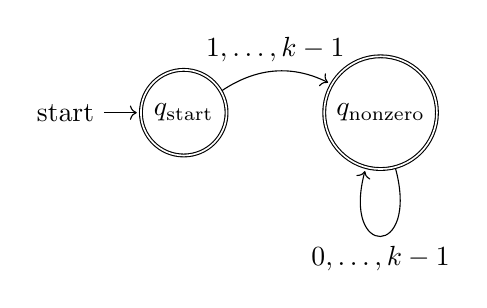
\begin{tikzpicture}[shorten >=1pt, node distance=2.5cm, on grid, auto]
            \node[state, initial, accepting] (q0) {$q_{\text{start}}$};
            \node[state, accepting] (q1) [right=of q0] {$q_{\text{nonzero}}$};
        
            % Transitions
            \path[->]
            (q0) edge[bend left] node[above] {$1,\dots,k-1$} (q1)
            (q1) edge[loop below] node {$0,\dots,k-1$} ()
            ;
        \end{tikzpicture}
    \end{center}
\end{solution}

\noindent \textbf{Exercise 5.3} \label{exercise5.3}: 

\begin{solution}
    % ¹²³⁴⁵⁶⁷⁸⁹⁰
    % suppose we have k = 10 and w = 1111, u = 2, v = 5
    % now we have   [uw]ₖ   =   21111 = 𝛼 10⁰ + 𝛽 
    %               [uvw]ₖ  =  251111 = 𝛼 10¹ + 𝛽 
    %               [uv²w]ₖ = 2551111 = 𝛼 10² + 𝛽 

    % suppose we have k = 2 and w = 3, u = 2, v = 5
    % now we have   [uw]ₖ   =  7 = 𝛼 2⁰ + 𝛽 
    %               [uvw]ₖ  = 21 = 𝛼 2¹ + 𝛽 
    %               [uv²w]ₖ = 59 = 𝛼 2² + 𝛽 

    Recall that we know for $\omega = d_m d_{m-1} \cdots d_0$, we have defined 
    \[ [\omega]_k = d_m k^m + d_{m-1} k^{m-1} + \cdots + d_1 k + d_0 \]
    Thus we can extend this definition and find that in general, we have 
    \begin{align*}
        [u v^n \omega]_k 
        & = [u]_k \cdot k^{n|v| + |\omega|} + [v]_k \cdot (1 + k^{|v|} + \cdots + k^{(n-1)|v|}) k^{|\omega|} + [\omega]_k \\ 
        & = [u]_k \cdot k^{n|v| + |\omega|} + [v]_k \cdot k^{|\omega|} \cdot \frac{k^{n|v|} - 1}{k^{|v|} - 1} + [\omega]_k \\ 
        & = \underbrace{ \left( [u]_k \cdot k^{|\omega|} + \frac{[v]_k \cdot k^{|\omega|}}{k^{|v|} - 1} \right) k^{|v|} }_{\alpha} \cdot k^{n} + \underbrace{ \left( - \frac{1}{k^{|v|} - 1} + [\omega]_k \right) }_{\beta} 
    \end{align*}
    the result is now obvious. 
\end{solution}

\noindent \textbf{Exercise 5.4} \label{exercise5.4}: 

\begin{solution}
    Similar to exercise 5.1 with the use of Fermat's Little Theorem. Suppose for a contradiction that the set $S$ is regular, thus it needs to satisfy the pumping lemma for some pumping length $p$. Find a prime $\gamma$ such that its base-$k$ expansion has length at least $p$, and can be written as $\gamma = uvw$. Therefore, by exercise 5.3, we kow that there exists integer $k$ and $\alpha$ and $\beta$ such that
    \begin{align*}
        [uvw]_k & = \alpha k + \beta \\ 
        [uv^nw]_k & = \alpha k^n + \beta 
    \end{align*} 
    Subtracting two equations yields us
    \[ [uv^nw]_k - [uvw]_k = \alpha ( k^n - k )  \]
    We can now pick $n = uvw$. By Fermat's Little Theorem, we know that RHS is divisible by $uvm$. Thus we can deduce that 
    \[ uvw \;|\; [uv^nw]_k \]
    which implies that $[uv^nw]_k \notin S$, contradiction. 
\end{solution}

\noindent \textbf{Exercise 5.5} \label{exercise5.5}: 

\begin{solution}
    This is similar to exercise 5.1. Suppose for a contradiction that the set of palindromes is regular, then there exists a pumping length $p$ satisfying the pumping lemma. Now consider an arbitrary string $\omega$ (palindrome) of length $2p + 1$, we know that in the decomposition $\omega xyz$, $xy$ does not contain the middle character of the palindrome $\omega$. As a result, it is now easy to see that the new string 
    \[ x y^i z \]
    wouldn't be a palindrome as desired, which further implies that $x y^i z \notin L$. This contradicts the pumping lemma, which means that that $L$ is not regular. 
\end{solution}

\noindent \textbf{Exercise 5.6} : 

\begin{solution}
    We denote the set of words over the alphabet $\{0, 1, \ldots, k-1\}$ that represent the base-$k$ expansions of elements of $\{\ell^n : n \geq 0\}$ as $L$. Suppose for a contradiction that $L$ does form a regular language. Hence for the pumping length $p$, let $\ell^n \in L$ be an element whose base-$k$ expansion has length at least $p$, suppose $\ell^n = uvw$, we have 
    \[ [uvw]_k = \alpha k + \beta = \ell^n \]
    for some rational numbers $\alpha$ and $\beta$. By the pumping lemma, we know that $uv^nw \in L$ for some $n \geq 0$ with $n \neq n'$, thus by exercise 5.3 we have 
    \[ [uv^nw]_k = \alpha k^n + \beta = \ell^{n'} \]
    for some $n'$. Subtracting the two equations we obtain that 
    \begin{align*}
        \ell^{n'} - \ell^n & = \alpha k^n - \alpha k \\ 
        n' \log \ell - n \log \ell & = \log \alpha + n \log k - \log \alpha - \log k \\ 
        n' \log \ell - n \log \ell & = n \log k - \log k \\ 
        (n' - n) \log \ell & = (n - 1) \log k
    \end{align*}
    This contradicts the fact that $\ell$ and $k$ are multiplicatively independent, hence the set of words does not form a regular language.  
\end{solution}

\noindent \textbf{Exercise 5.7a} : 

\begin{solution}
    Suppose for a contradiction that $L$ is regular. Hence for a fixed pumping length $p$, we can find $\ell \in L$ with $|\ell| \geq p$ such that $\ell = xyz$. We assume that $|\ell| = q$ for some prime $q$. By the pumping lemma, we know that 
    \[ x y^{q + 1} z \in L \]
    However, it is easy to see that $q \;|\; | xy^{q+1}z |$, a contradiction. Hence $L$ is not regular. 
\end{solution}

\noindent \textbf{Exercise 5.7b} : 

\begin{solution}
    Unmatched number of left and right parentheses. 
\end{solution}

\noindent \textbf{Exercise 5.8} : 

\begin{solution}
    
\end{solution}

\noindent \textbf{Exercise 5.9} : 

\begin{solution}
    
\end{solution}

\newpage

\noindent \textbf{Exercise 7.1} : 

\begin{solution}
    \texttt{(a) $\Rightarrow$ (b)}: We define 
    \[ A = \begin{bmatrix}
        0 & 1 & 0 & \cdots & 0 \\ 
        0 & 0 & 1 & \cdots & 0 \\ 
        \vdots & \vdots & \vdots & \ddots & \vdots \\ 
        0 & 0 & 0 & \cdots & 1 \\ 
        -c_0 & -c_1 & -c_2 & \cdots & -c_{d-1} 
    \end{bmatrix} \quad \text{ and } \quad \mathbf{w}= \begin{bmatrix}
        f(0) \\ f(1) \\ \vdots \\ f(d-1) 
    \end{bmatrix} \]
    We prove by induction on $n$ that 
    \[ \begin{bmatrix}
        f(n) \\ f(1) \\ \vdots \\ f(d-1) 
    \end{bmatrix} = A^n \mathbf{w} \] 
    For our base case, we know by the definition of $\mathbf{w}$ that 
    \[ \begin{bmatrix}
        f(0) \\ f(1) \\ \vdots \\ f(d-1) 
    \end{bmatrix} = A^0 \mathbf{w} \] 
    Suppose the result holds for $m < n$. Now we have 
    \begin{align*}
        A^n \mathbf{w} = A A^{n-1} \mathbf{w} 
        & = A \begin{bmatrix}
            f(n-1) \\ f(n-1+1) \\ \vdots \\ f(n-1+d-1) 
        \end{bmatrix} = \begin{bmatrix}
            f(n) \\ f(n+1) \\ \vdots \\ f(n+d-1) 
        \end{bmatrix}
    \end{align*}
    as desired. For the other direction \texttt{(b) $\Rightarrow$ (a)}: Recall that from Cayley-Hamilton we know that 
    \[ A^d + c_{d-1} A^{d-1} + \cdots + c_1 A + c_0 I = 0 \]
    Hence we further know that 
    \[ \mathbf{v} \left( A^{n+d} + c_{d-1} A^{n+d-1} + \cdots + c_1 A^{n+1} + c_0 A^n \right) \mathbf{w} = 0 \]
    which yields us the recurrence relation of the form in statement (a). 
\end{solution}

\newpage

\noindent \textbf{Exercise 7.2} : 

\begin{solution}
    \texttt{(a) $\Rightarrow$ (c)}: We define 
    \[ Q(x) := 1 + c_{d-1} x + \cdots + c_0 x^d \]
    and 
    \[ P(x) := \left( \sum_{n \geq 0} f(x) x^n \right) \cdot Q(x) \]
    Thus it now suffices to show that $P(x)$ is a polynomial of degree at most $d - 1$. We notice that 
    \[ [x^m] P(x) = \sum_{i = 0}^{\min(m, d)} c_{d - i} \cdot f(m - i) \]
    Given that $f(n)$ satisfies a linear recurrence:
    \[
    f(n + d) + c_{d-1} f(n + d - 1) + \cdots + c_0 f(n) = 0 \quad \text{for all } n \geq 0
    \]
    Then, for any $m \geq d$, we have:
    \[ f(m) + c_{d-1} f(m - 1) + \cdots + c_0 f(m - d) = 0 \]
    This implies:
    \[ [x^m] P(x) = f(m) + c_{d-1} f(m - 1) + \cdots + c_0 f(m - d) = 0 \qquad \text{for all } m \geq d \] 
    thus proving that $P(x)$ has degree at most $d - 1$. For the other direction, \texttt{(c) $\Rightarrow$ (a)}: Suppose we know that 
    \[ \sum_{n \geq 0} f(n) x^n = \frac{P(x)}{Q(x)} \] 
    Hence we know 
    \[ [x^i] Q(x) \sum_{n \geq 0} f(n) x^n \] 
    Suppose 
    \[ Q(x) = c_d x^0 + c_{d-1} x + \cdots + c_0 x^d \]
    where $c_d = 1$ since $Q(0) = 1$, we now have that 
    \begin{align*}
        [x^i] Q(x) \sum_{n \geq 0} f(n) x^n
        & = [x^i] \sum_{j = 0}^d c_{d-j} x^j \sum_{n \geq 0} f(n) x^n \\ 
        & = \sum_{j = 0}^d c_{d-j} [x^{i-j}] \sum_{n \geq 0} f(n) x^n = \sum_{j = 0}^d c_{d-j} f(i-j)
    \end{align*}
    Moreover, given that $P(x)$ is a polynomial of degree at most $d-1$, we know that 
    \[ [x^d] P(x) = 0 \]
    which implies that 
    \[ [x^d] Q(x) \sum_{n \geq 0} f(n) x^n = \sum_{j = 0}^d c_{d-j} f(d-j) = 0 \]
    as desired. 
\end{solution}

\newpage

\noindent \textbf{Exercise 7.3} : 

\begin{solution}
    \texttt{(c) $\Rightarrow$ (d)}: We may factor 
    \[ Q(x) = (1 - \lambda_1 x)^{p_1} \cdots (1 - \lambda_e x)^{p_e} \]
    for some nonnegative integer $e \leq d$, given $Q(0) = 1$. Hence we know that 
    \begin{align*}
        
    \end{align*}
\end{solution}

\newpage

\noindent \textbf{Exercise 7.4} : 

\begin{solution}
    We first show that $\displaystyle \sum_{d|n} \mu(d) = \begin{cases}
        1 & n = 1 \\ 0 & n \neq 1
    \end{cases}$. It is easy to see that when $n = 1$, we indeed have $\mu(1) = 1$. For all the other cases, suppose the number $n$ has $m$ distinct prime factors $p_1, \ldots, p_m$, thus we know that 
    \[ \sum_{d|n} \mu(d) = \sum_{j = 0}^m (-1)^j \binom{m}{j} = (1 + (-1))^m = 0 \]
    Now, we have \begin{align*}
        \sum_{d|n} \mu(d) f(n/d) 
        & = \sum_{d|n} \mu(d) \sum_{m| n/d} g(m) \\ 
        & = \sum_{m|n} g(m) \sum_{d| n/m} \mu(d)
    \end{align*}
    Notice the only term that is non-zero for the right-hand side summation is when $m = n$, hence we have 
    \[ \sum_{d|n} \mu(d) f(n/d) = g(m) = g(n) \]
    as desired. 
\end{solution}

\noindent \textbf{Exercise 7.5} : 

\begin{solution}
    We notice that every word of length $n$ is built by repeating a primitive word of length $d$, where $d|n$, hence we have 
    \[ k^n = \sum_{d|n} f(d) \]
    Using möbius inversion we obtain that 
    \[ f(n) = \sum_{d|n} \mu(d) k^{n/d} \]
    as desired. 
\end{solution}

\noindent \textbf{Exercise 7.6} : 

\begin{solution}
    We have 
    \begin{align*}
        \sum_{n \geq 0} f(n) x^n 
        & = f(0) x^0 + \sum_{n \geq 1} f(n) x^n \\ 
        & = 1 + \sum_{n \geq 1} \sum_{d|n} \mu(d) k^{n/d} x^n \\ 
        & = 1 + \sum_{d \geq 1} \mu(d) \sum_{j \geq 1} k^{j} x^{dj} \\ 
        & = 1 + \sum_{d \geq 1} \mu(d) \frac{kx^d}{1 - kx^d}
    \end{align*}
    \hl{which is a little different from what we wanted.}
\end{solution}

\noindent \textbf{Exercise 7.7} : 

\begin{solution}
    By Theorem 6.4, we know that if a language $L$ is regular, then the number of length-$n$ words in $L$ satisfy some recurrence relation. Therefore, it suffices to prove that the expression we obtained in Exercise 7.6 isn't an expansion of a rational function to conclude that the set of primitive words over a $k$-letter alphabet is not a regular language. 


\end{solution}




\end{document}